\chapter{Organization}


\section{Project Management System}
In order to achieve our project on schedule we had to define steps to optimize the management of our time and to avoid delay on deadline.
%\paragraph{Step 1}
During early months at the launch of project, we started by writing the user requirements, which is a document etablished according to the need of the product owner. The user requirements allowing all users to orient the project progress and to keep in view the expected objectives. So this is a writing task. This  user requirements was presented to the product owner and before an academic jury.
This was about getting validation on user requirements of the product owner so that we make sure that his needs are clearly understood by us.
\paragraph{}
Then we had, thanks to Mister Chatelier's training a project manangement system called scrum. This system was about detailling all the tasks there was to complete and specifically the sprints.
\\In this part, we will describe the organization of our work throughout the project and will  present  tools used to the  project management.
%\paragraph{Step 2}
\newpage
For the project management,we used the Backlog and the Trello.
\subsection{ Backlog}
Thanks to the training given by Mister Christian Chatellier, we define the implementation of the project management system.
\\This system includes the backlog writing which listseach individual task there is to complete during the project and affords us to define every sprints (knowing that a sprint represents a week of work).
\\In the backlog all tasks are classified by priority and if a task contained in the backlog does not contribuate to the project objectives ,we must remove it
\begin{figure}[bth]%[!ht]
\begin{center}
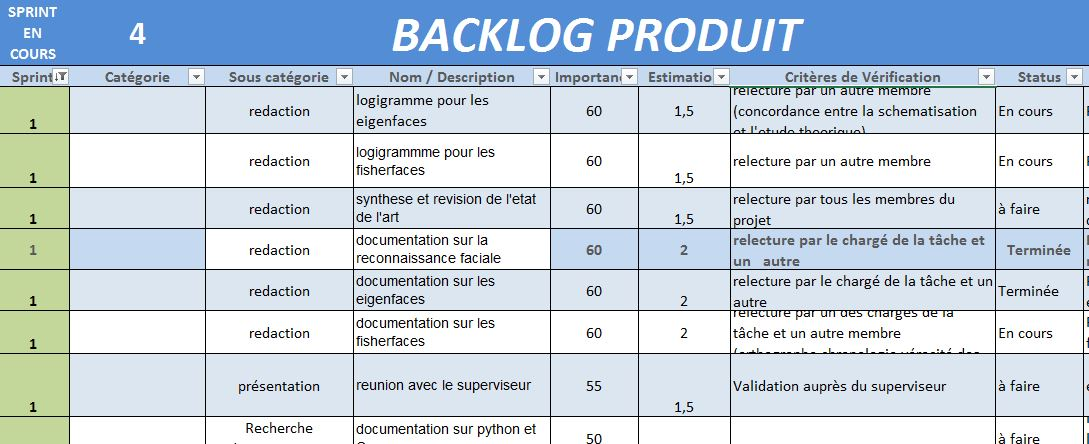
\includegraphics[scale=0.60]{baclog}%[height=70mm,width=70mm]
\caption{\textbf{Backlog}}%
%\url {http://www.google.fr/}
%\label{learningPhaseGM}
\end {center}
\end{figure}
\paragraph{}
In the backlog ,we have many parameters:
\begin{itemize}
\item Sprint:current sprint of a moment( a sprint correspond to a week)
\item Subcategory :  category of a task (redaction,research,programming or meeting with the product owner)
\item Name/description: description of a task
\item Importance : priority of task
\item estimation : time or duration for a task
\item criteria for verification
\item Status : indicates the status of a  task(doing,done)
\end{itemize}
Note that every friday we change the priority of certains tasks for praparing the next sprint.
\newpage
\subsection{Trello}
\subsubsection{Presentation}
The second tool used is Trello
Trello  is a project management tool allowing to list all project tasks.It is composed by many cards.
\\ With Trello we launch the scrum  every morning by a meeting between members of the group projet.It enables to see the progress work for all member  of the project.
\\our Trello is divides  into five cards:
\begin{itemize}
\item To do :list of all tasks that we have to do for  the week
\item Doing: list of current  tasks (Task  for a day)
\item Wait :tasks  waiting for very precise reasons
\item Test and Validation : task done but not yet tested
\item Done : Completed Tasks 
\end{itemize}
Note also that the project is divided into several weeks each corresponding to a Sprint.
\subsubsection{Sprint}
There we present the four sprint of the project :
\begin{itemize}
\item Sprint 1 
\\For this sprint we complete a second part which is the writing of the state of art. A document reporting the theoretical aspect to be developped in the project but also the explanation of the methods used and the algorithms to be programmed.During this sprint all intended tasks  have been completed
\begin{figure}[bth]%[!ht]
\begin{center}
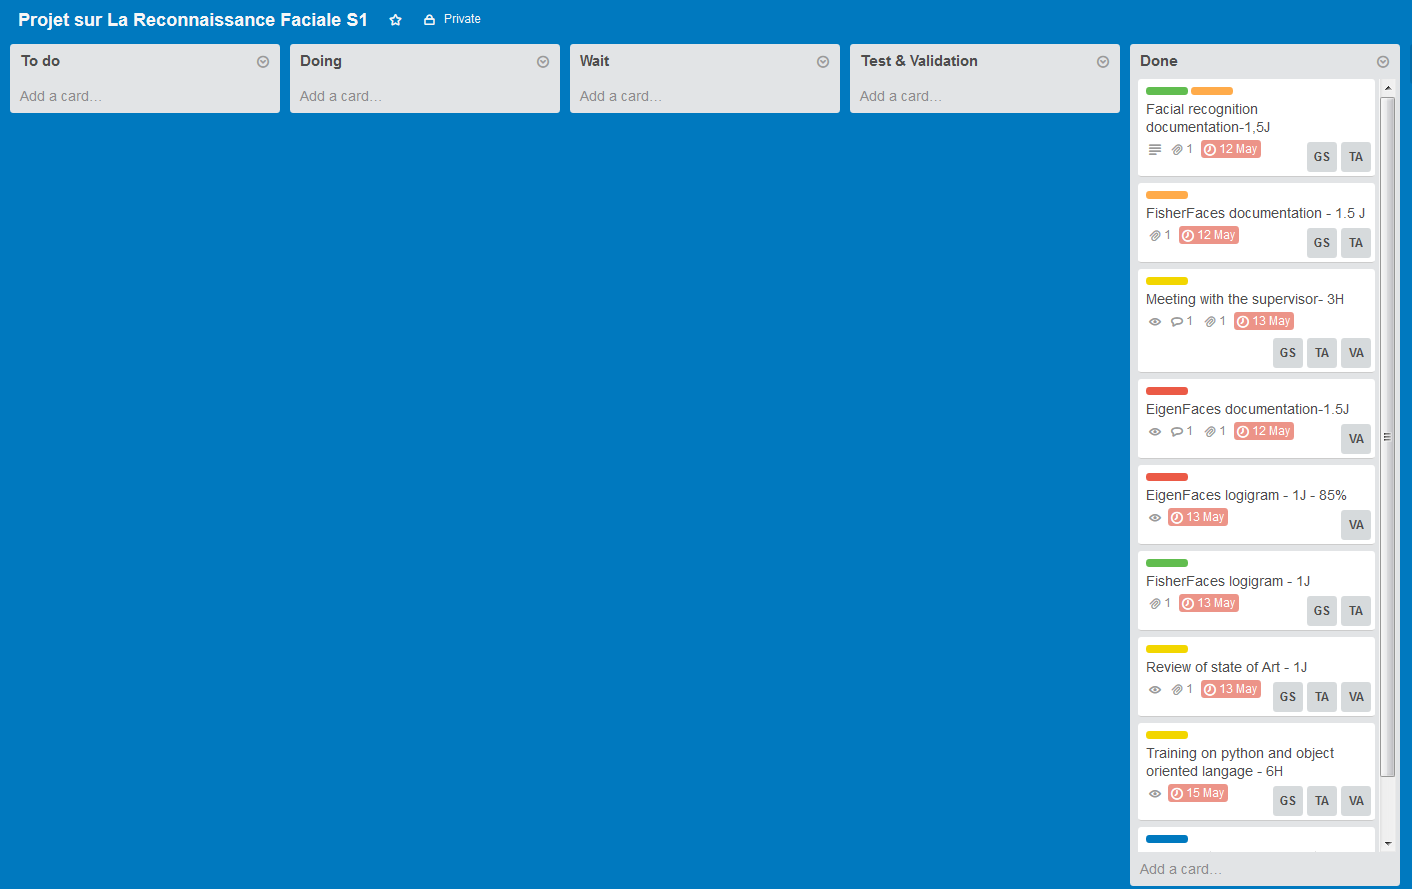
\includegraphics[scale=0.60,height=10cm,width=17cm]{sprint1}
\caption{\textbf{First sprint }}%
%\url {http://www.google.fr/}
%\label{learningPhaseGM}
\end {center}
\end{figure}
\newpage
\item Sprint 2 
\\At  the sprint 2, we did a literature search to deepen the appearance of algorithmic methods and presented the results of our research so that we all stand on the same point of view.We begin the prototype for eigenfaces method  in python. 
\begin{figure}[bth]%[!ht]
\begin{center}
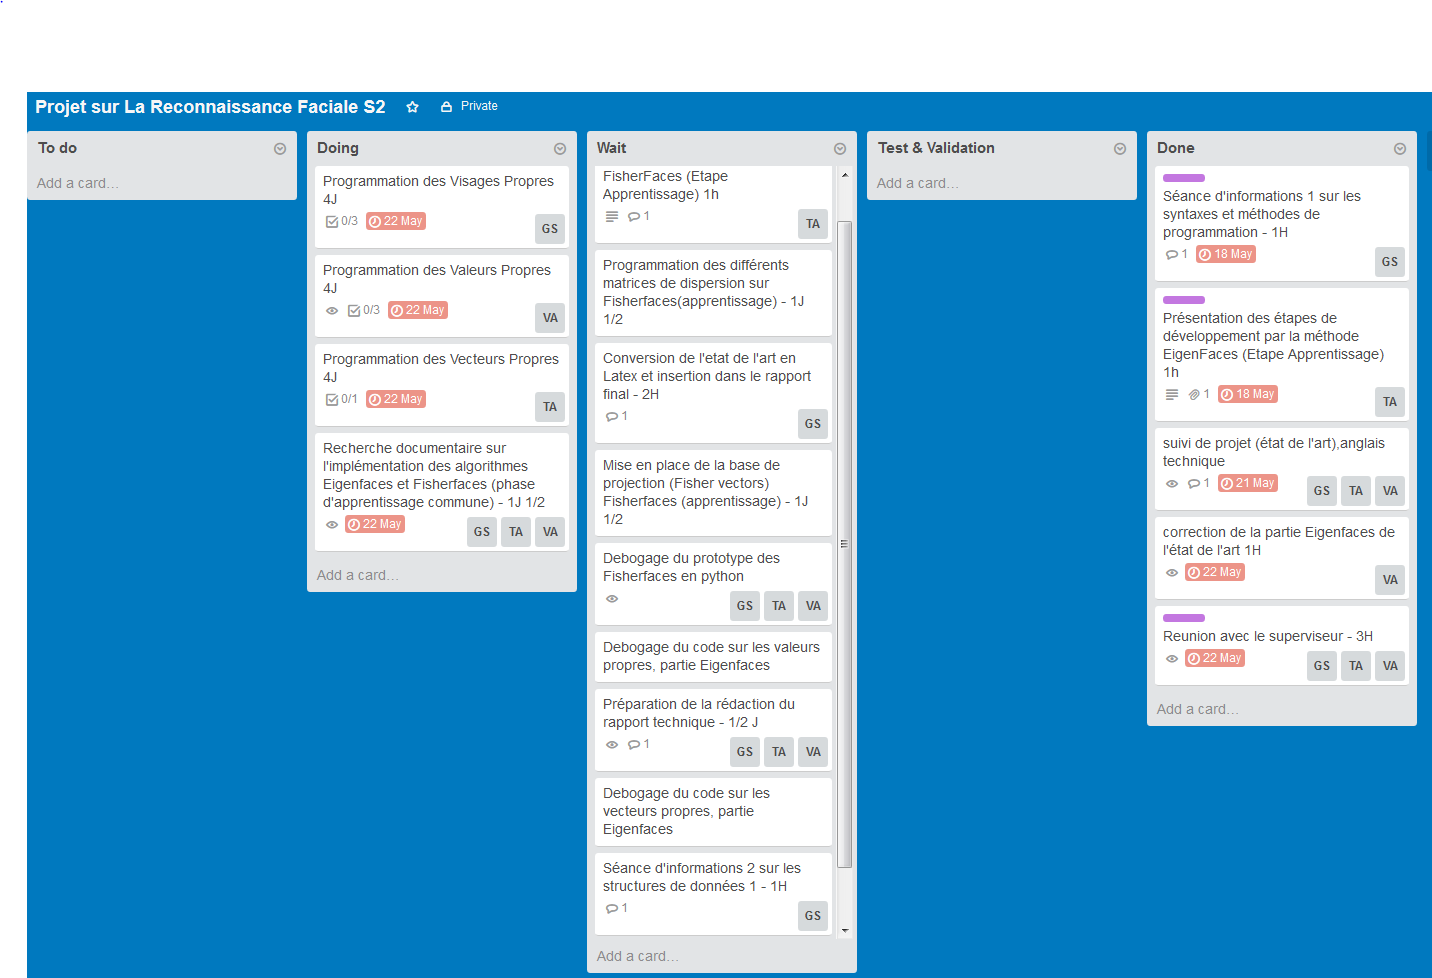
\includegraphics[scale=0.60,height=15cm,width=17cm]{sprint2}
\caption{\textbf{Second sprint }}%
%\url {http://www.google.fr/}
%\label{learningPhaseGM}
\end {center}
\end{figure}
\newpage
\item Sprint 3
\\This sprint consists in finishing the previous tasks started in later sprint about programming eigenfaces method. But added to those tasks we scheduled in the writing tasks. By the way some of the programming tasks  uncompleted  are renewed in Sprint 4.
\begin{figure}[bth]%[!ht]
\begin{center}
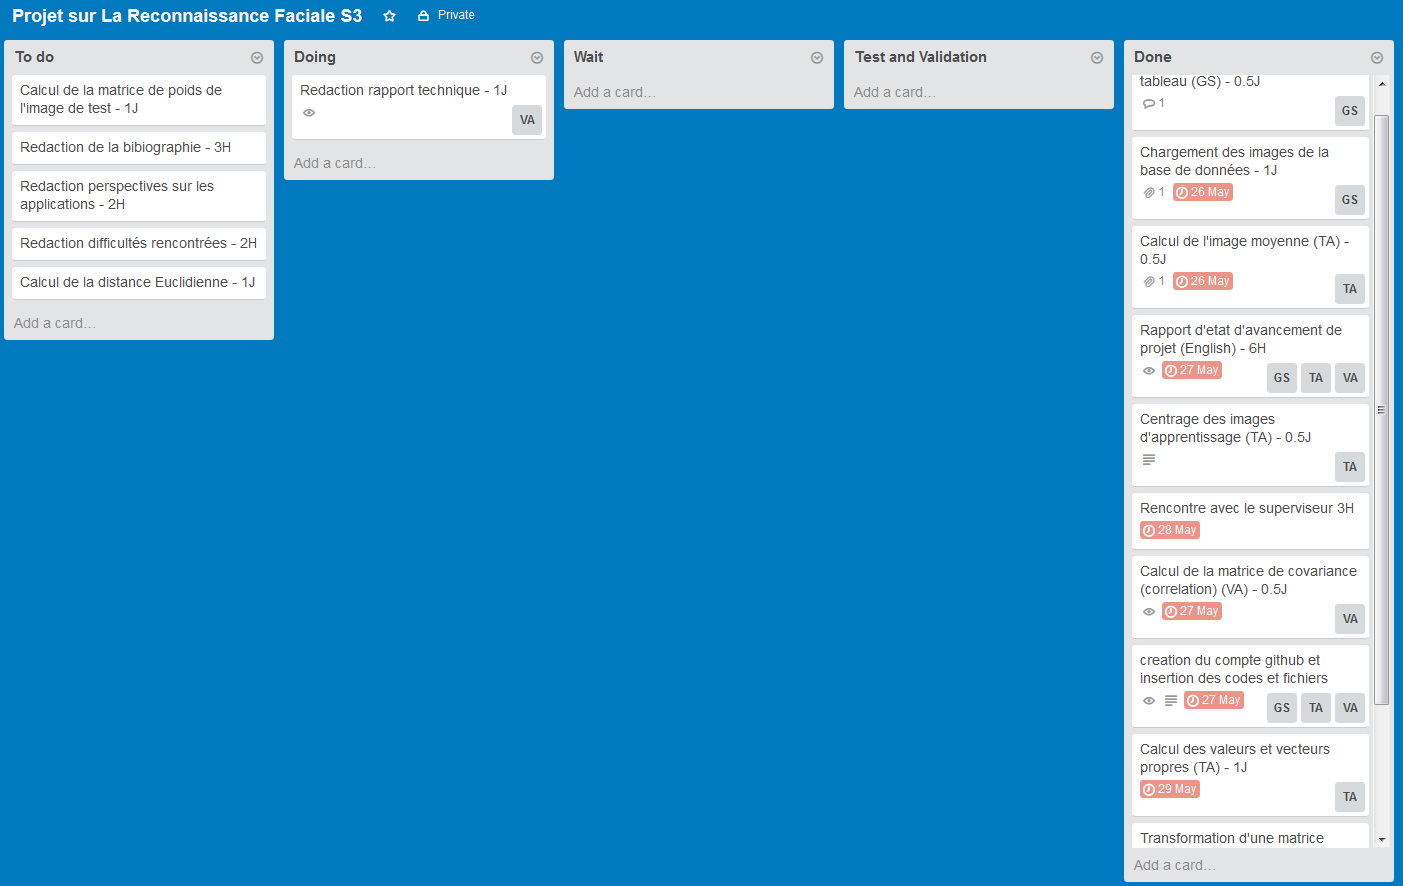
\includegraphics[scale=0.60,height=15cm,width=17cm]{sprint3}
\caption{\textbf{Third sprint }}%
%\url {http://www.google.fr/}
%\label{learningPhaseGM}
\end {center}
\end{figure} 
\newpage 
\item Sprint 4
\\For this sprint, we started by programming  Fisherfaces method but did not stop us to progress on the eigenfaces method.We also achieved some writting tasks.
\begin{figure}[bth]%[!ht]
\begin{center}
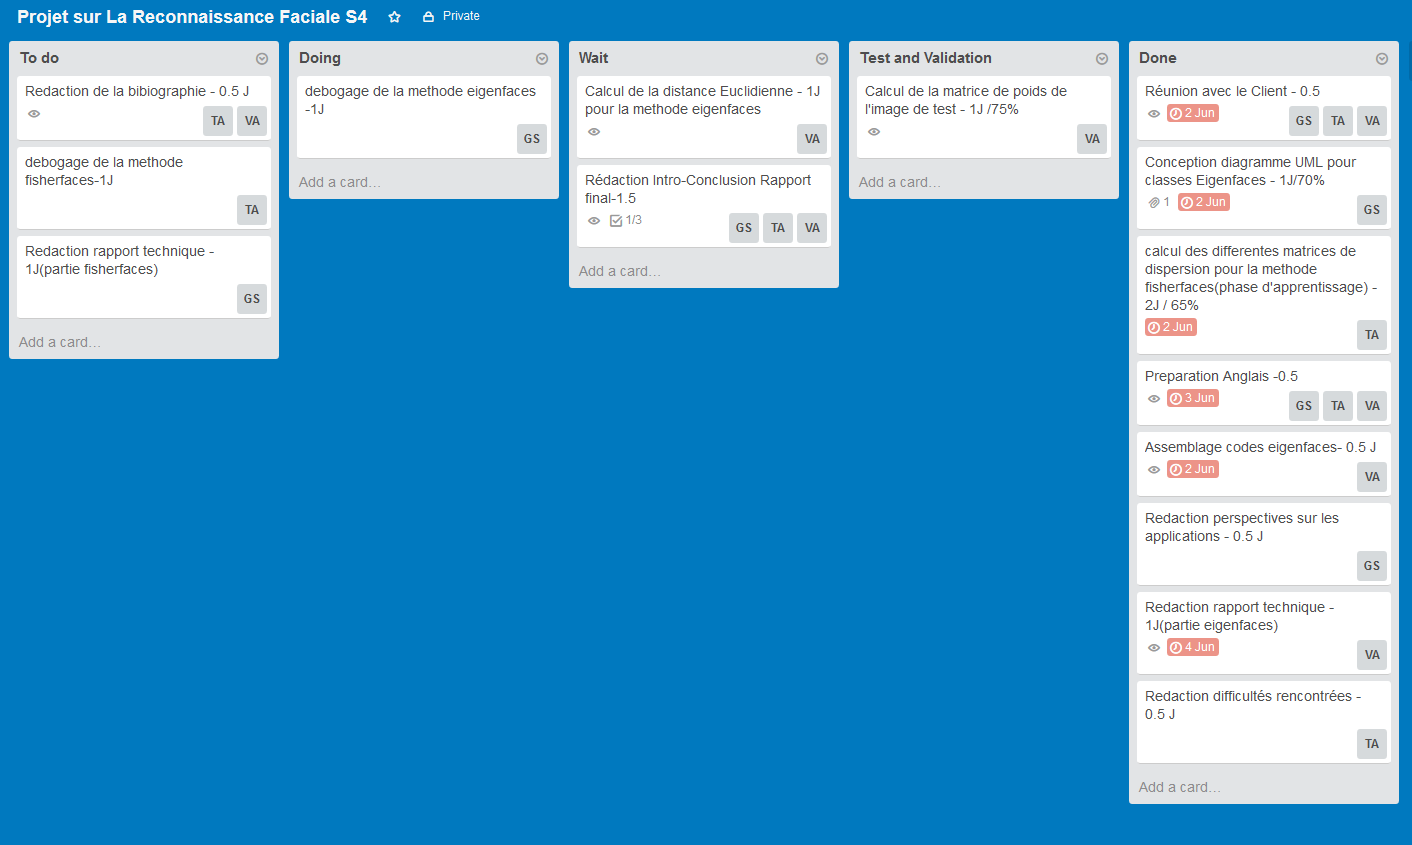
\includegraphics[scale=0.60,height=15cm,width=17cm]{sprint4}
\caption{\textbf{fourth sprint }}%
%\url {http://www.google.fr/}
%\label{learningPhaseGM}
\end {center}
\end{figure}


\end{itemize}

\clearpage
\section{Team Project}

The sponsor of this project is M. Pascal Bourdon working for XLIM-SIC Laboratory in Poitiers as a researcher. The results will be used by the Laboratory.
\paragraph{}
The project team includes :

Supervisors:
\begin{itemize}
\item	Pascal BOURDON as Supervisor and Product Owner;
\item	David HELBERT as Academic Training Principle;
\item	Christian CHATELLIER as Project Management Supervisor.
\end{itemize}
Students in charge:
\begin{itemize}
\item	Viviane Arame BASSE as Communication Manager
\item	Guy Florent A. SADELER as Technical Manager
\item	Ali TOILHA as Project Manager
\end{itemize}
The End users of this project are:
\begin{itemize}
\item	XLIM-SIC Laboratory,
\item	RTMA Training of the University of Poitiers for tutorials,
\item	Product owner and any potential company requiring facial recognition technology.
\end{itemize}
% Obvisoulsy, a Trello account was created from that document to allow us to hold a daily project meeting whiwh lasts fifteen minute and is called Scrum. Scrum is useful for daily monitoring of the current sprint.




%\paragraph{Step 3}
%Once, an organization detailling progressively every single task there is to complete and the different %actor on it we could more easily work on the programming part of our project to program the prototypes.